\section{STM Version Manual}
\subsection{Read the time}
\begin{center}
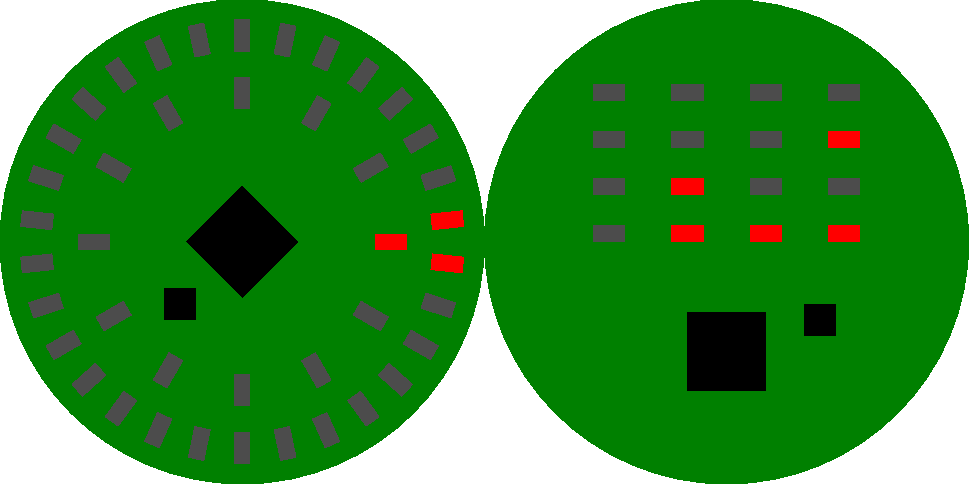
\includegraphics[width=0.6\textwidth]{../Graphics/Time3_15}
\end{center}
To read the Watch it is necessary to activate the Display this can be either done via double tapping the Housing or raising the arm to take a look on the watch(tilt it by a minimum of 12 degrees with the Watchface facing up and holding it steady for about one second)

\paragraph{Analog}
The analog Version an be read equally to a normal Watch. 
In the inner Ring the Hours from 1 to 12 are displayed. 
In the outer Ring the minutes are displayed from 0 to 59, 
since there are only 30 LEDs in the outer ring for uneven minutes the nearest two LEDs are lit up. 
For example for 3:15 the LEDs signalling 14 and 16 are lit up.

\paragraph{Binary}
in the Binary Version the LEDs are read columnwise as BCD code starting with 1 at the bottom. So the right two columns are showing the Minutes. If an LED is litone have to add its Value to the Minutes if not then nothing is added. So for the full hour no led in the right two columns will be lit.
In the example above in the first column no LED is lit. In the second column the LED for 1 and 2 are lit. In the third column the LED for 1 is lit and in the last column the LED for 1 and 4 are lit.
So it is 3:15.
\subsubsection{setting the Time}
To enter the Time setting mode you have to turn the Watch in show time mode upside down, Watchface facing the ground an double Tap it. The Watch enters debouncing mode.
In debouncing mode the Hours 80 and Minutes 80 are blinking for the binary version for the Analog Version Hours 12 and 6 are blinking. (Blinking leds are displayed brighter in the graphic.
\begin{center}
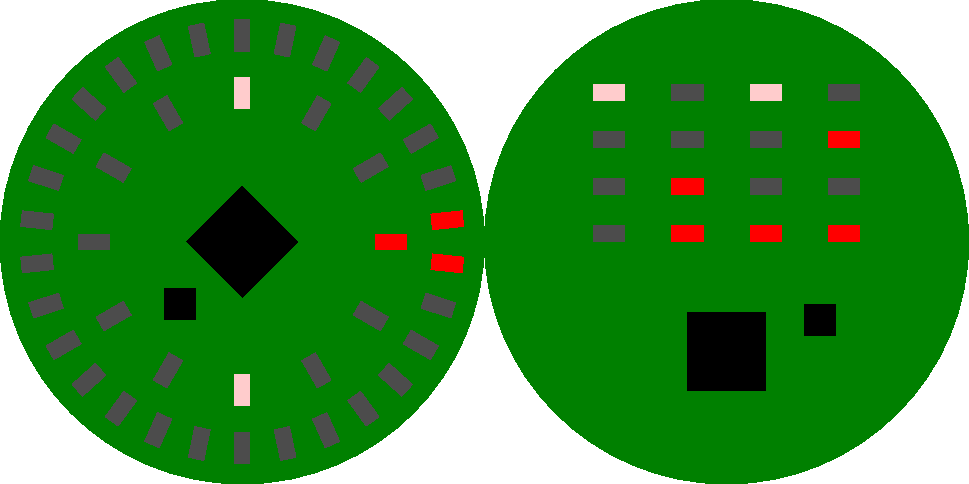
\includegraphics[width=0.6\textwidth]{../Graphics/Time3_15_debouncing}
\end{center}
While in debouncing mode turn the watch around again (Watchface facing up)  and double Tap it again to enter Set Hour mode.
\begin{center}
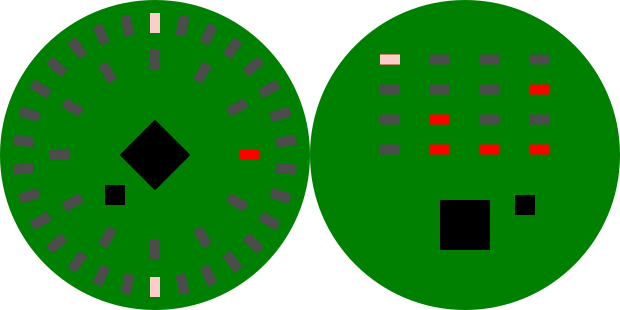
\includegraphics[width=0.6\textwidth]{../Graphics/Time3_15_SetHour}
\end{center}
In the set hour mode the hour can be increased by leaning the Watch away from you and decreased by leaning the watch towards you.
Once the hour is set correctly double Tap the Watch again to enter Set Minute Mode.
\begin{center}
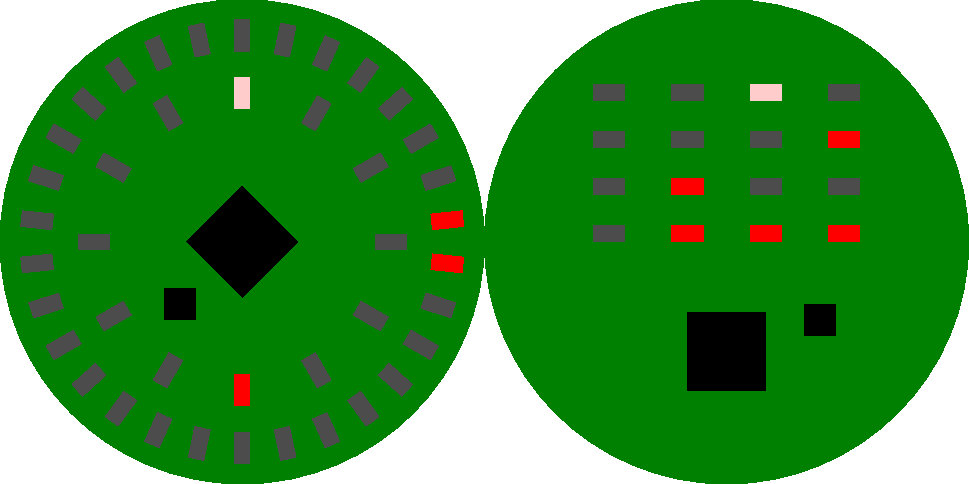
\includegraphics[width=0.6\textwidth]{../Graphics/Time3_15_SetMinute}
\end{center}
The Set hour mode works exactly like to set hour mode. Increasing and decreasing is done via leaning the Watch fowrward an backward. Once finished a double Tap sets the Seconds to 0 and starts the Watch again.
\subsection{Read the Date}
\begin{center}

\includegraphics[width=0.6\textwidth]{../Graphics/Date25_Dez}
\end{center}
To enter the Date display mode tilt the Watch in Time Mode to the Front(Facing away from you) at least 10 degrees and double Tap it.
\paragraph{Analog}
On the analog Version The Minutes 40 and 50 are lit up to signal Date Display.
On the Hours Ring the Month is displayed as Hour and the Day is Displayed as Minutes.

\paragraph{Binary}
On the binary Version the first column is showing 3 to signal Date Display.
In the second and third column the Day is displayed as BCD Code and the Month is displayed in binary code(it does not stop on 9)\\
\\
A double Tap with the watch facing up switches back to show time mode.

\subsubsection{setting the Date}
To enter the Date setting mode you have to turn the Watch in show date mode upside down, Watchface facing the ground an double Tap it. The Watch enters debouncing mode.
In debouncing mode the Hours 8 and Minutes 80 are blinking for the binary version for the Analog Version Minutes 40 and 50 are blinking. (Blinking leds are displayed brighter in the graphic.
\begin{center}
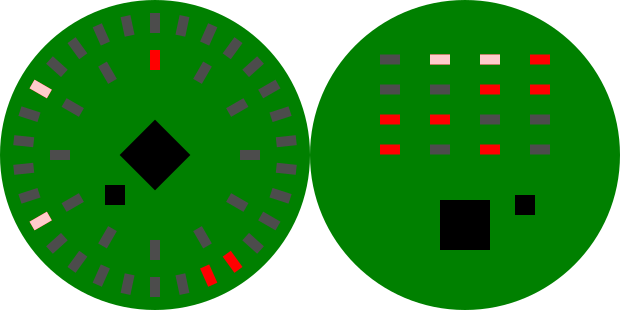
\includegraphics[width=0.6\textwidth]{../Graphics/Date25_Dez_debouncing}
\end{center}
While in debouncing mode turn the watch around again (Watchface facing up)  and double Tap it again to enter set day mode.
\begin{center}
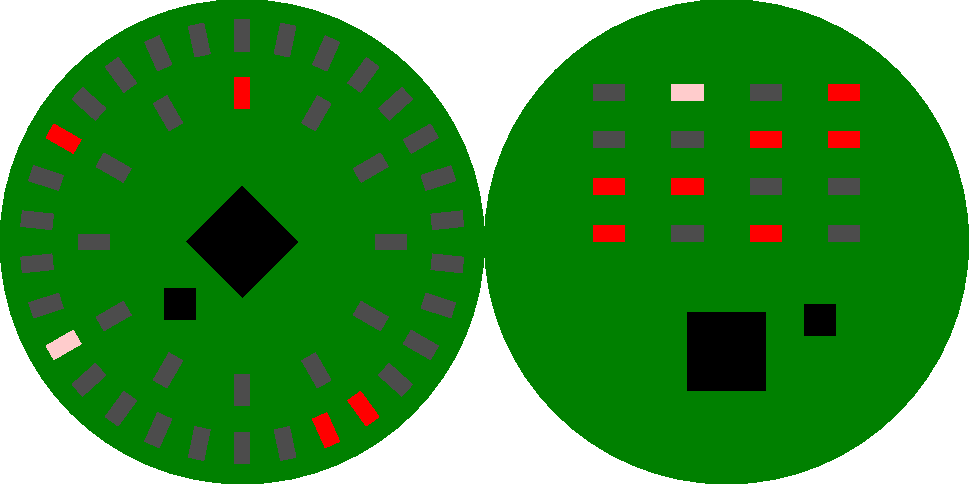
\includegraphics[width=0.6\textwidth]{../Graphics/Date25_Dez_SetDay}
\end{center}
Setting the Day works exactly like setting the hour. Increasing and decreasing is done via leaning the Watch fowrward an backward. Once finished a double Tap switches to set month mode.
\begin{center}
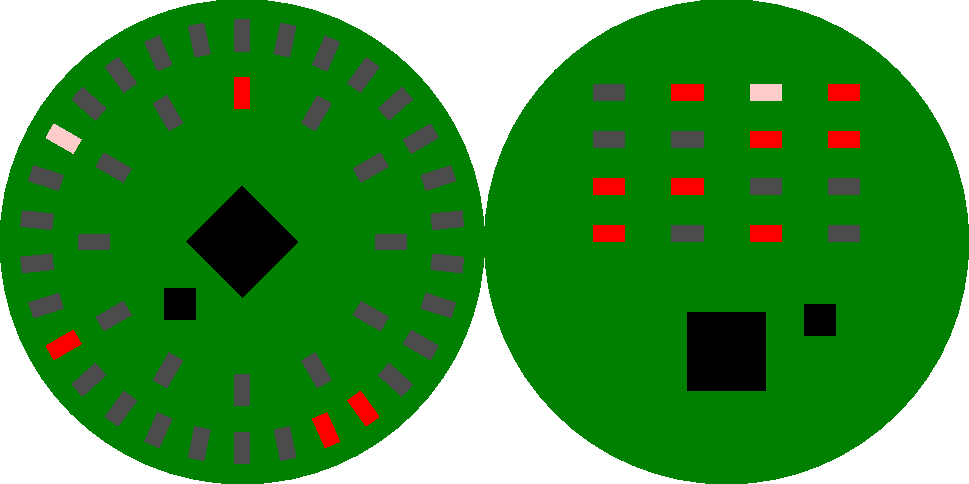
\includegraphics[width=0.6\textwidth]{../Graphics/Date25_Dez_SetMonth}
\end{center}
Setting the Month works exactly like setting the hour. Increasing and decreasing is done via leaning the Watch fowrward an backward. Once finished a double Tap switches to set year mode.
\begin{center}
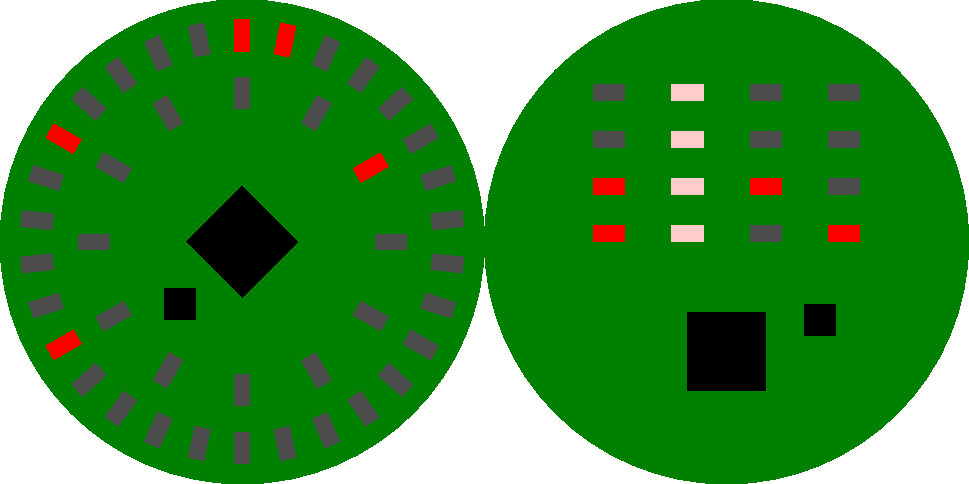
\includegraphics[width=0.6\textwidth]{../Graphics/Date25_Dez_SetYear21}
\end{center}
The year is only used for the leap year calculation and can be only set between 0 and 99. 
\paragraph{Analog} 
In the Analog Version the Set year mode is signalized by blinking both minute LEDs 30 and 50. The Year tens are shown in the inner ring with one LED per Counter and the ones are shown in the outer ring with one LED per counter. In this example XX21.
\paragraph{Binary}
Setting Year mode is displayed by showing 3 in the first column and blinking all LEDs in the second column. The year is displayed in columns 3 and 4. In this example XX21.\\
\\
Setting the Month works exactly like setting the hour. Increasing and decreasing is done via leaning the Watch fowrward an backward. Once finished a double Tap sets the Seconds to 0 and starts the Watch again.
\subsection{Todays Steps}
\begin{center}
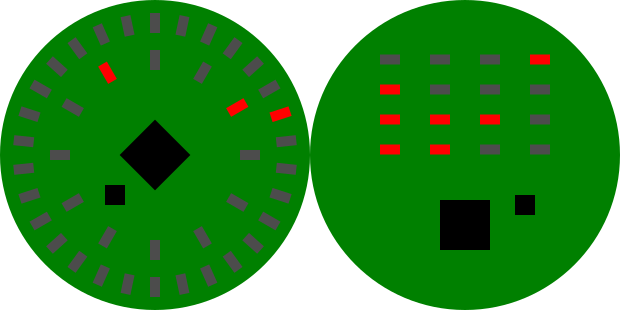
\includegraphics[width=0.6\textwidth]{../Graphics/ShowSteps32768}
\end{center}
To enter Step display mode tilt the Watch in Time Mode to the Back(Facing you) at least 10 degrees and double Tap it.
\paragraph{Analog}
On the Analog Watch the hour LED 11 is lit up with the overflow counter (from 0(12 o'clock) to 3. The overflow counter counts the number of whole rounds on the Stepcounter. An overflow occurs on 15000. The current Stepcounter without overflow is displayed in the outer Ring. Each LED signalizes 500 Steps. The value is rounded to 500.
In the Example the overflow counter shows 2 and the counter itself shows 6.
$2*15000+6*500 = 33000$
\paragraph{Binary}
On the binary Watch the Step Counter is signalized by the forst column showing 7. Column 2 to 4 shows the steps in 100 counts rounded to 100 counts. So 32768 in the exmample will be shown as (7)328\\
\\
A double Tap with the watch facing up switches back to show time mode.

\subsection{Show steps history}
To enter the steps history mode you have to turn the Watch in show steps mode upside down, Watchface facing the ground an double Tap it.
\begin{center}
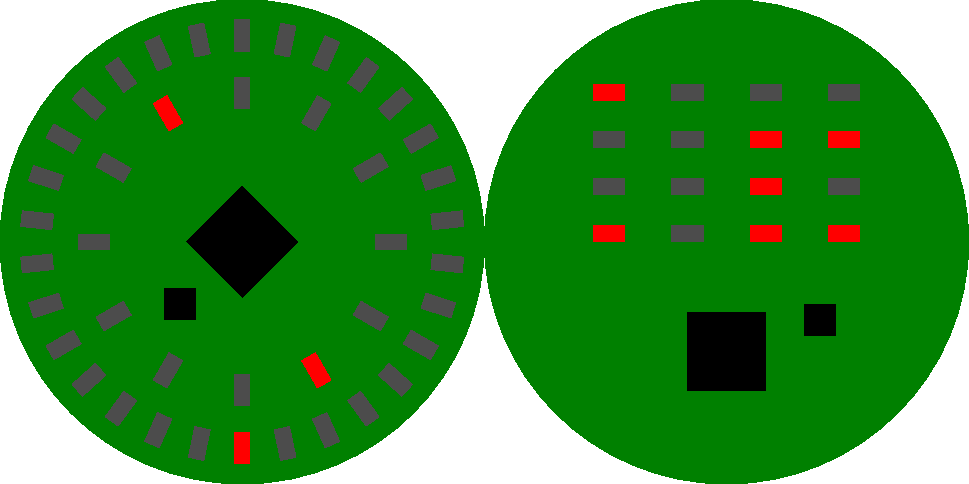
\includegraphics[width=0.6\textwidth]{../Graphics/ShowStepsHist_2Days_ago_7500}
\end{center}
The history counter can be increased and decreased by leaning the watch back and forth.
\paragraph{Analog} 
The steps history mode looks like the Show steps mode, but there is an additional LEDas Hitory Counter lit up. The History counter starts at Hour 4 and increases depending on how far ago the Date is. In the Example Hour 5 is shown, so the history is from 2 days ago. The steps are show as in the Show Steps mode, so there were 7500 Steps done two days ago.
\paragraph{Binary}
The steps hitory mode is signalized by the H80 LED. The LEDs below show how long ago the Steps were counted, the counter starts yesterday with 0. so the example shows the Data from 2 Days ago. The steps are displayed as in the show steps mode. so the example shows 7500 Steps 2 days ago.\\
\\
to leave this mode double tap changes to the show Battery Voltage.
\subsection{show battery voltage}
To enter the steps history mode you have to double tap the Watch in show steps history mode.
\begin{center}
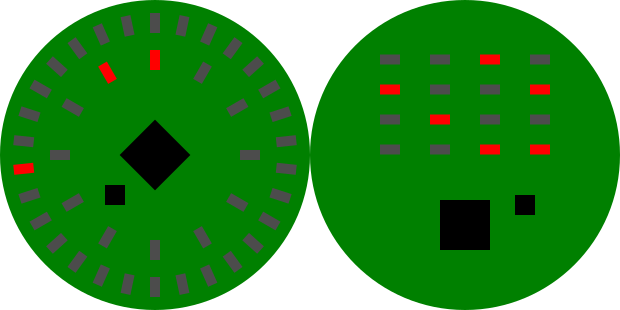
\includegraphics[width=0.6\textwidth]{../Graphics/ShowUBatt_2950mV}
\end{center}
\paragraph{Analog}
The show battery voltage is signalized by the Hour 11 and 12 lighting up together. The voltage is shown on the minutes ring, scaled from 3.5V to 1,5V, so each quarter is 0,5V. The Watch in the example is showing 2,95V.

\paragraph{Binary}
The show battery voltage is signalized by the Hour 40 LED. Column 2 to 4 are showing the Battery voltage in 10mV granularity. So the Example shows $2950mV=2,95V$\\
\\
A double Tap with the watch facing up switches back to show steps mode.